\subsection{Einführung}

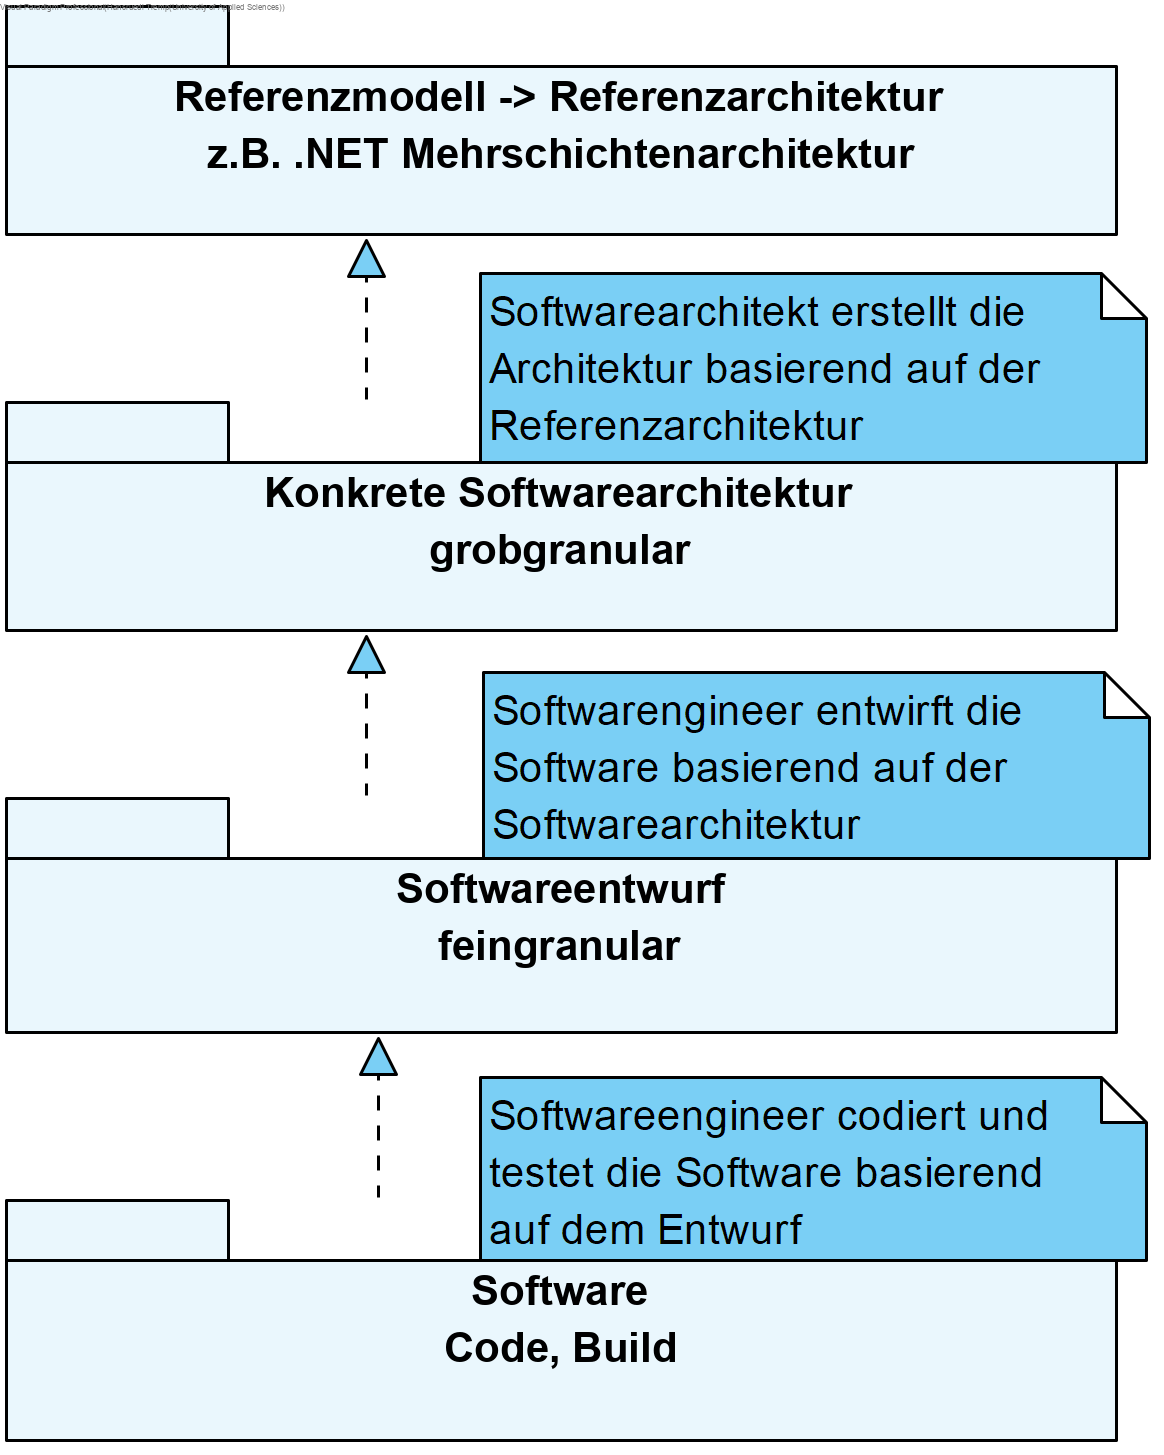
\includegraphics[width=0.7\linewidth]{introduction-arch-roles.png}

\subsubsection{Ebenen}

\textbf{Referenzmodell}

legt grundlegende Begriffe und Prinzipien fest (Bsp. .NET, Jakarta EE) \\

\textbf{Referenzarchitekturen}

Wenden \textcolor{blue}{Referenzmodelle} an und geben Musterarchitekturen vor (Bsp. Mehrschichtenarchitektur, IoT-Architektur) \\

\textbf{Softwarearchitektur} Wird basierend auf der
\textcolor{blue}{Referenzarchitektur} erstellt (Bsp. Mobile Native-App mit REST-Zugriff auf Web-Server), grobgranular, Darstellung oft mit \textcolor{blue}{UML-Klassendiagramm}

\textbf{Softwareentwurf}
Legt feingranulare Struktur fest (Bsp. Aufbau der Native-App: GUI - Funktionsebenen - Zugriff auf Server), feingranular, Darstellung oft mit \textcolor{blue}{UML-Klassendiagramm}

\subsubsection{Rollen}
\textbf{Enterprise/IT-Architekt}

Referenzmodell $\rightarrow$ Referenzarchitektur

\begin{itemize}
    \item Referenzmodell ist Leitfaden für Referenzarchitektur
    \item Baut Referenzarchitektur basierend auf dem Domänenverständnis des Referenzmodells
\end{itemize}
\vspace{10pt}
\textbf{Softwarearchitekt}

Referenzarchitektur $\rightarrow$ Konkrete Architekturen

\begin{itemize}
    \item Erstellt die Architektur basierend auf der Referenzarchitektur
    \item Legt grundlegende Strukturen fest
\end{itemize}
\vspace{10pt}
\textbf{Softwarengineer}

Konkrete Architekturen $\rightarrow$ Konkrete Systeme

\begin{itemize}
    \item Entwirft die Software basierend auf der Softwarearchitektur (grobgranular)
    \item Codiert und testet die Software basierend auf dem Entwurf (feingranular)

\end{itemize}

\subsubsection{Ziele}

\textbf{SMART}

\begin{itemize}
    \item \textcolor{blue}{Spezifisch}, konkret, fassbar
    \item \textcolor{blue}{Messbar}, testbar, später überprüfbar
    \item \textcolor{blue}{Akzeptiert} von (möglichst) allen Stakeholdern
    \item \textcolor{blue}{Realistisch}, aus aktueller Ressourcensicht machbar
    \item \textcolor{blue}{Terminiert} im Rahmen des Projektplanes
\end{itemize}
\vspace{10pt}
\textbf{Architekt (Person)}

Stabile \textcolor{blue}{Lösungskonzepte} für eine Reihe von technischen Aspekten liefern, damit Entwickler die Qualitätsziele erreichen. \\

\textbf{Architektur}

Ziel der Softwarearchitektur ist die Sicherstellung einer
adäquaten \textcolor{blue}{Softwareproduktequalität}.

\begin{itemize}
    \item \textcolor{blue}{Nützlichkeit} Applikation erfüllt ihre Funktionen
    \item \textcolor{blue}{Festigkeit} Software ist stabil und langlebig
    \item \textcolor{blue}{Ästhetik} User Experience ist ansprechend
\end{itemize}
\vspace{10pt}

\subsubsection{Anforderungen}
\textbf{Satzschablone}

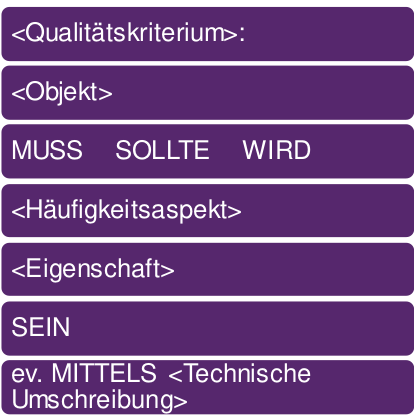
\includegraphics[width=0.6\linewidth]{introduction-satzschablone.png}

Beispiele
\begin{itemize}
    \item \textcolor{blue}{Verfügbarkeit} Das IT-System MUSS > 90 \% voll funktionstüchtig SEIN MITTELS passender Hardware und Netzwerkanbindung.
    \item \textcolor{blue}{Zeitverhalten} Die Antwort vom System MUSS in 80 \% der Fälle max. 2 Sec. SEIN
    \item \textcolor{blue}{Zeitverhalten} Die Antwort vom System SOLLTE in 90 \% der Fälle max. 1 Sec SEIN
    \item \textcolor{blue}{Interoperabilität} Das Austauschformat zwischen den Microservices WIRD immer JSON SEIN.
\end{itemize}
\vspace{10pt}
\textbf{ISO 25010 Softwarequalitätsmodell}

Benutzer

\begin{itemize}
    \item Funktionalität
    \item Performance und Effizienz
    \item Kompatibilität und Interoperabilität
    \item Benutzbarkeit
    \item Verfügbarkeit
\end{itemize}

Betreiber/Entwickler

\begin{itemize}
    \item IT-Sicherheit
    \item Warbarkeit
    \item Portierbarkeit
\end{itemize}


\subsubsection{Struktur (Modellierung)}

Hilft für

\begin{itemize}
    \item Beherrschung der Komplexität
    \item Architektur gestalten und kommunizieren
    \item Verständigung mit Stakeholdern
    \item Dokumentation und Nachvollziehbarkeit gewährleisten
\end{itemize}
\vspace{10pt}
\textbf{Bausteine}

\begin{itemize}
    \item \textcolor{blue}{Pakete} Fassen untergeordnete Pakete bzw. Komponenten zu einer Einheit zusammen (Bsp. in Schichten).
    \item \textcolor{blue}{Komponenten} Klar definiertes Verhalten und bieten Schnittstellen an oder Konsumieren diese über Beziehungen
\end{itemize}
\vspace{10pt}
\textbf{Diagramme}

\textcolor{blue}{Kontextsicht} zeigt den Scope des Systems mit den Schnittstellen

\begin{itemize}
    \item Kontextdiagramm \\
    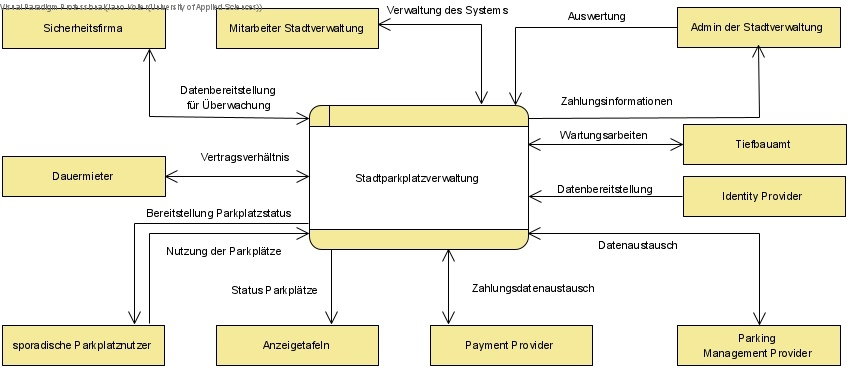
\includegraphics[width=\linewidth]{introduction-context-diagram.png}
    \item Use Case Diagramm
\end{itemize}

\textcolor{blue}{Bausteinsicht} zeigt strukturellen Aufbau des Systems

\textcolor{blue}{Laufzeitsicht} zeigt dynamische Aspekte, wie Interkation, Prozessablauf und Verhalten

\begin{itemize}
    \item Sequenzdiagramm
    \item Aktivitätsdiagramm
    \item Zustandsdiagramm
\end{itemize}

\textcolor{blue}{Verteilungssicht} zeigt die Verteilung der Softwareartefakte in der IT-Infrastruktur

\begin{itemize}
    \item Deployment Diagram
\end{itemize}

\subsubsection{Prüfungsfragen}

\begin{itemize}
    \item Erläutern Sie die Aufgabe der Softwarearchitektur im Rahmen eines Softwareentwicklungsprojektes! \\
    \textcolor{blue}{Der Softwarearchitekt gibt anhand
    einer Referenzarchitektur die Architekturvorgaben. Er hilft unteranderem mit, die Architekturrichtlinien und -standards in der IT-Strategy zu entwickeln. Zusätzlich ist der für die Kommunikation mit den Stakeholdern zuständig.}
    \item Welche Beziehung hat die Softwarearchitektur zur Referenzarchitektur einerseits und dem Softwarentwurf andererseits? \\
    \textcolor{blue}{Die Softwarearchitektur ist eine konkrete Anwendung einer Referenzarchitektur und bildet die Vorlage für den feingranularen Softwareentwurf.}
    \item Welche konkreten Artefakte erstellt der Softwa-
    rearchitekt? \\
    \textcolor{red}{Antwort}
    \item Welches sind die drei Hauptziele in der Analogie mit der klassischen Bauarchitektur? \\
    \textcolor{blue}{Nützlichkeit, Festigkeit, Ästhetik}
    \item Wozu dient arc42? \\
    \textcolor{blue}{Vorlage für die Dokumentation}
    \item Mit welchem Diagrammtyp von UML können sie die Struktur eines Softwaresystems beschreiben? \\
    \textcolor{blue}{Komponentendiagramm}
    \item Wozu dient ein UML Komponentendiagramm? \\
    \textcolor{blue}{Darstellung des strukturellen Aufbaus, sowie die Beziehungen der Komponenten}
    \item Nennen Sie drei der wichtigsten Werkzeuge eines Softwarearchitekten! \\
    \textcolor{blue}{Wiki, Modellierungstools, Analysetools und Testtools}
\end{itemize}
